\documentclass{exam}
\usepackage[exos]{main}

\title{Longueurs de courbes}
\date{4 Avril 2024}
\author{Seconde 9}

\begin{document}
\maketitle

\section{Introduction}
Les exercices suivants posent la question : Comment mesurer la longueur de la courbe représentative d'une fonction ? À quoi une telle mesure peut bien servir ?
\vspace*{0.5cm}
\begin{questions}
\question On se donne la fonction carrée 
\begin{equation*}
\function{f}{\left[0;10\right]}{\R}{x}{x^2}
\end{equation*}
\begin{parts}
\part Vérifier que les points $A(0;0)$, $B(5;25)$ et $C(10;100)$ sont des points de la courbe représentative de $f$, $\mathcal{C}_f$.
\part Calculer la longueur des segments $[AB]$ et $[BC]$.
\part En déduire la longueur de la ligne brisée représentée ici.
\begin{center}
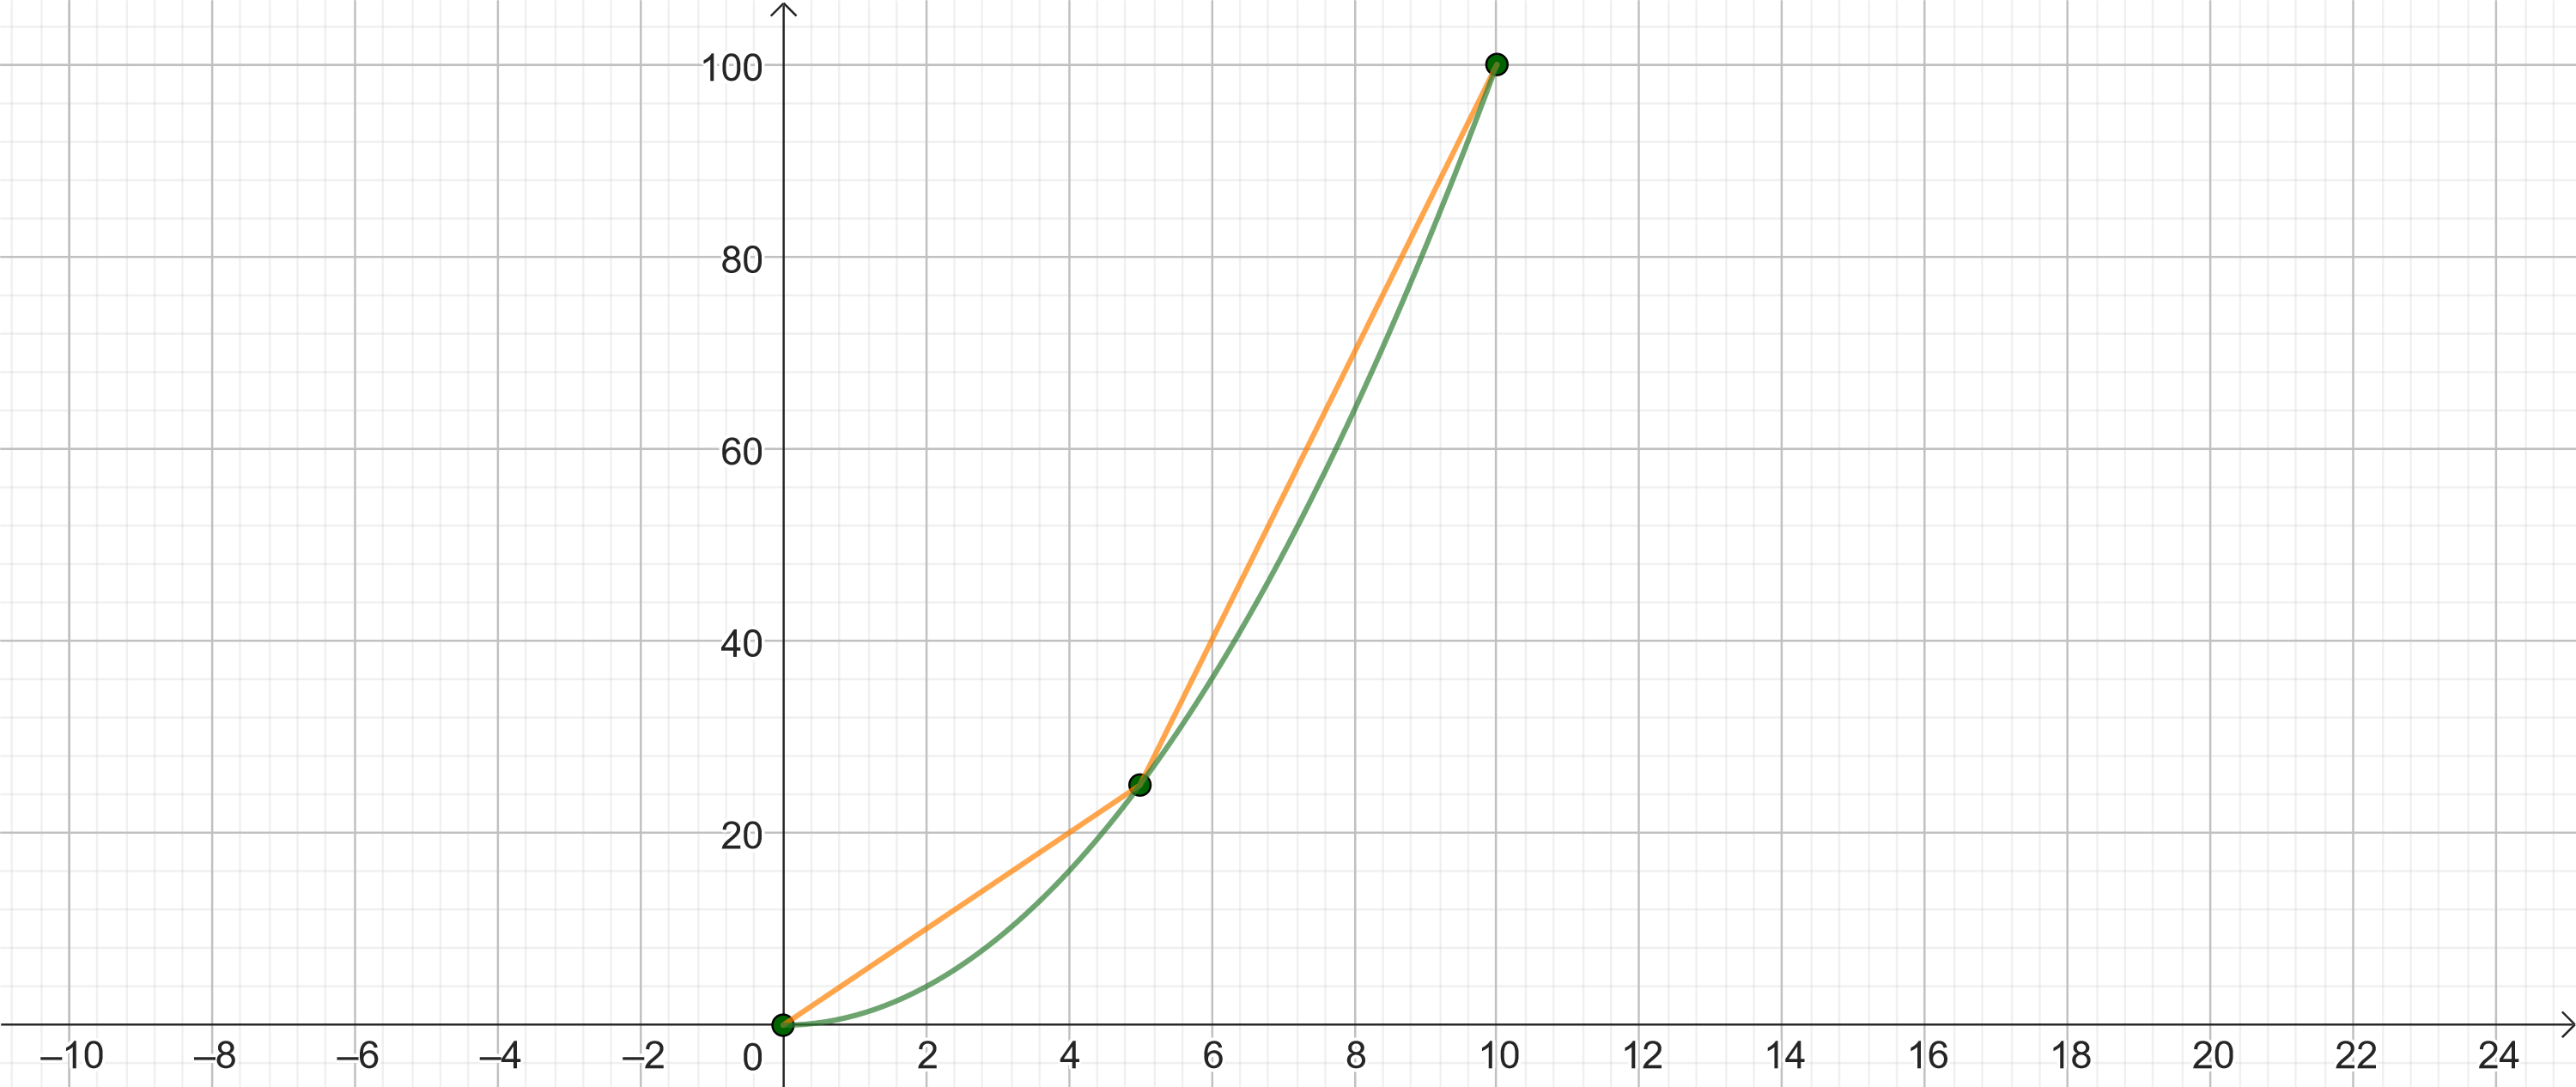
\includegraphics[scale=0.5,trim={0 0 7cm 0},clip]{fonctionCarre.png}
\end{center}
\part Refaire le même travail, mais avec les points
\begin{itemize}
\item $A(0;0)$
\item $B(2;4)$
\item $C(4;16)$
\item $D(6;36)$
\item $E(8;64)$
\item $F(10;100)$
\end{itemize}
Faire un schéma représentant la courbe représentative de $f$ ainsi que la ligne brisée $ABCDEF$. Cette longueur vous parait-elle une meilleure approximation de la longueur de la courbe ?
\part Proposer une méthode pour obtenir une approximation encore meilleure.
\end{parts}
\newpage
\question On s'intéresse maintenant à la fonction
\begin{equation*}
\function{g}{[-1;1]}{\R}{x}{\sqrt{1 - x^2}}
\end{equation*}
\begin{parts}
\part La courbe représentative $\mathcal{C}_g$ est représentée ci-après.
\begin{center}
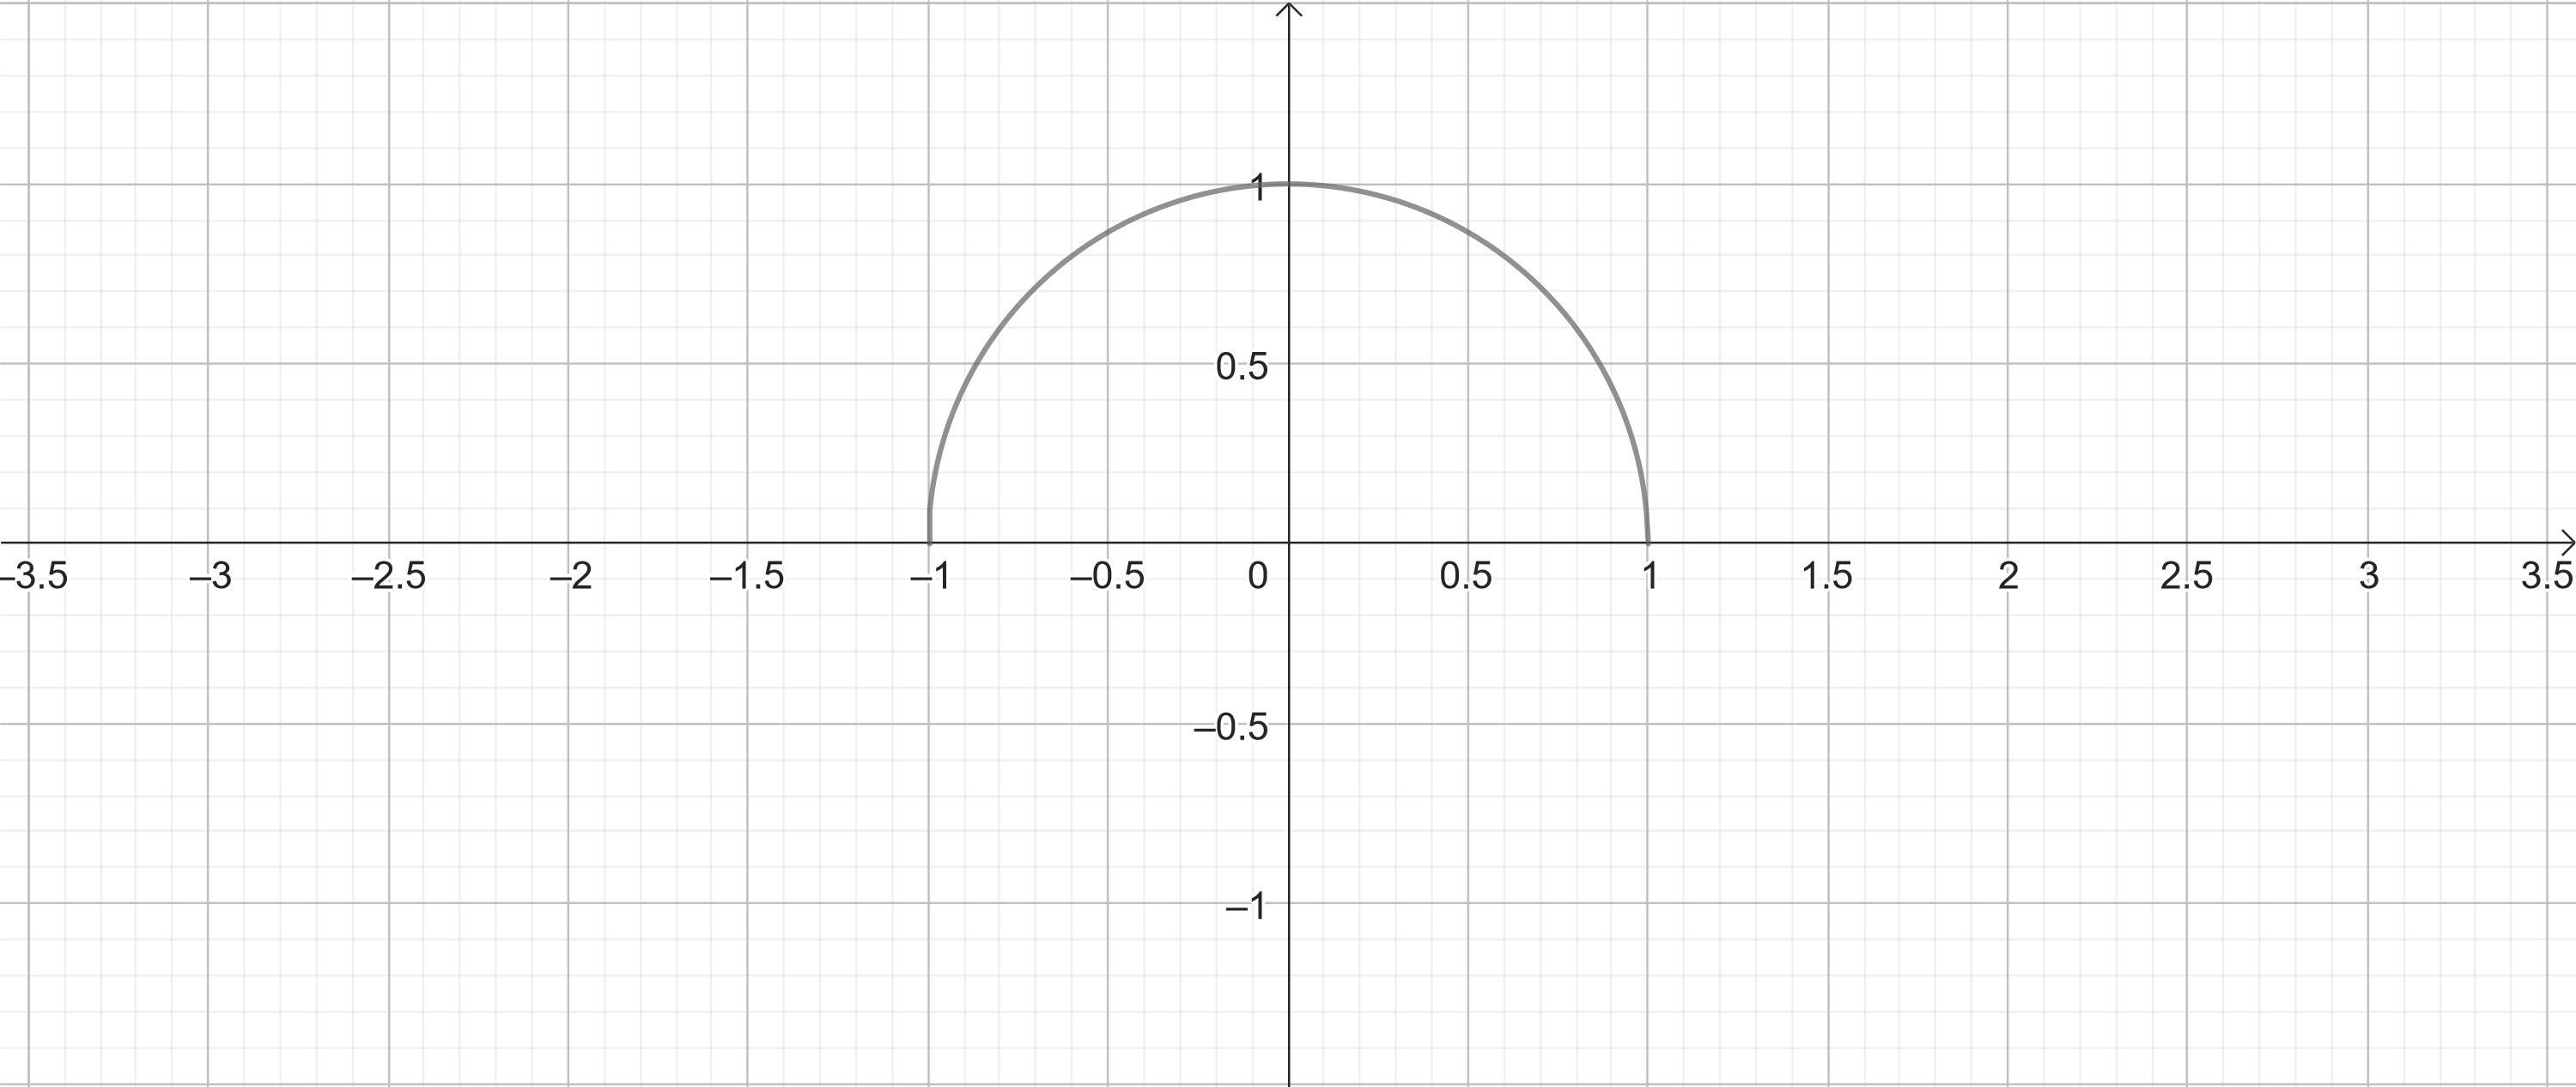
\includegraphics[width=15cm]{fonctionCercle.png}
\end{center}
À quoi ressemble cette courbe ?
\part Montrer que pour tout $x \in \left[-1;1\right]$, le point $M(x,g(x))$ appartient au cercle de longueur $1$ et de centre $O(0,0)$.
\part En déduire la longueur de cette courbe.
\part En vous inspirant du premier exercice, proposer une méthode pour approximer une valeur numérique de $\pi$. Appliquer cette méthode en utilisant les points
\begin{itemize}
\item $A(-1;0)$ 
\item $B(-0,5;\sqrt{0,75})$ 
\item $C(0;1)$ 
\item $D(0,5;\sqrt{0,75})$ 
\item $E(1;0)$ 
\end{itemize}
\end{parts}
\end{questions}
\end{document}